\begin{figure}[tb]
\centering
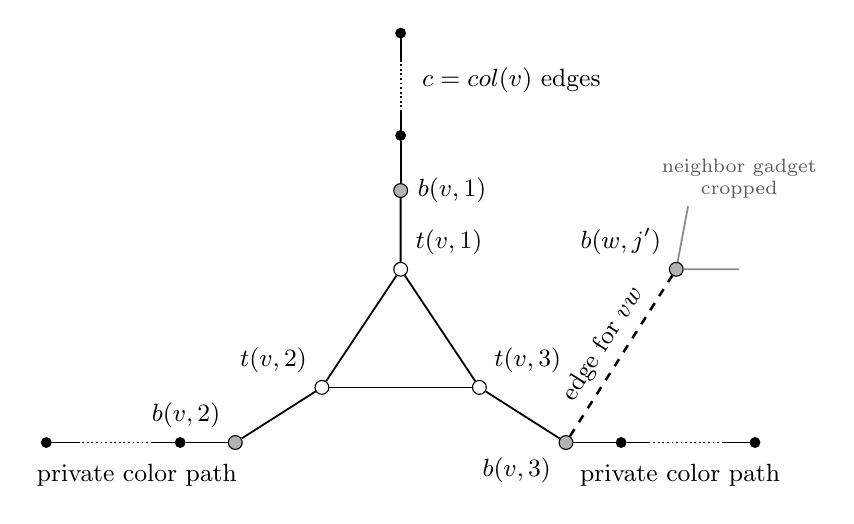
\begin{tikzpicture}[
  x=1cm,y=1cm,
  font=\small,
  vertex/.style={
    circle,draw,fill=white,inner sep=0pt,minimum size=5pt
  },
  connector/.style={vertex,fill=black!30},
  pathvertex/.style={vertex,fill=black,minimum size=3.5pt},
  graph edge/.style={line width=.65pt},
  external edge/.style={
    graph edge,dashed,line width=.9pt
  }
]
  \node[vertex,label=above right:{$t(v,1)$}] (t1) at (0,1) {};
  \node[vertex,label=above left:{$t(v,2)$}] (t2) at (-1,-.5) {};
  \node[vertex,label=above right:{$t(v,3)$}] (t3) at (1,-.5) {};
  \draw[graph edge] (t1)--(t2);
  \draw[graph edge] (t2)--(t3);
  \draw[graph edge] (t3)--(t1);
  \node[connector,label=right:{$b(v,1)$}] (b1) at (0,2) {};
  \node[connector,label=above left:{$b(v,2)$}]
    (b2) at (-2.1,-1.2) {};
  \node[connector,label=below left:{$b(v,3)$}]
    (b3) at (2.1,-1.2) {};
  \draw[graph edge] (t1)--(b1) (t2)--(b2) (t3)--(b3);

  \node[pathvertex] (p11) at (0,2.7) {};
  \node[pathvertex] (p1c) at (0,4) {};
  \draw[graph edge] (b1)--(p11)--(0,3);
  \draw[graph edge,densely dotted] (0,3)--(0,3.65);
  \draw[graph edge] (0,3.65)--(p1c);
  \node[right] at (.15,3.4)
    {$c=\operatorname{col}(v)$ edges};

  \node[pathvertex] (p21) at (-2.8,-1.2) {};
  \node[pathvertex] (p2c) at (-4.5,-1.2) {};
  \draw[graph edge] (b2)--(p21)--(-3.15,-1.2);
  \draw[graph edge,densely dotted]
    (-3.15,-1.2)--(-4.1,-1.2);
  \draw[graph edge] (-4.1,-1.2)--(p2c);
  \node[pathvertex] (p31) at (2.8,-1.2) {};
  \node[pathvertex] (p3c) at (4.5,-1.2) {};
  \draw[graph edge] (b3)--(p31)--(3.15,-1.2);
  \draw[graph edge,densely dotted]
    (3.15,-1.2)--(4.1,-1.2);
  \draw[graph edge] (4.1,-1.2)--(p3c);
  \node[below] at (-3.35,-1.35) {private color path};
  \node[below] at (3.55,-1.35) {private color path};

  \node[connector,label=above left:{$b(w,j')$}]
    (bw) at (3.5,1) {};
  \draw[external edge]
    (b3)--node[midway,above,sloped] {edge for \(vw\)} (bw);
  \draw[graph edge,black!45]
    (bw)--(3.65,1.8)
    (bw)--(4.3,1);
  \node[font=\scriptsize,black!65,align=center]
    at (4.3,2.15) {neighbor gadget\\cropped};
\end{tikzpicture}
\caption{The uncoloring gadget at a vertex \(v\).
Each triangle member has its own connector and each connector
has a private path of exactly \(c=\operatorname{col}(v)\) edges.
Dotted portions abbreviate path interiors; for \(c=1\), each private
path is a single pendant edge.
The dashed edge represents an original edge \(vw\) attached at its
chosen ports.  In this schematic example \(b(v,3)\) uses its external
port, while \(b(v,1)\) and \(b(v,2)\) do not.
The neighboring gadget is cropped, with its connector's other two
incidences shown as short stubs.
Shading and line styles explain the construction and are not graph
colors or additional relations.}
\label{graph:fig-uncoloring}
\end{figure}
